\begin{frame}
	\begin{itemize}\justifying
		\item How many boolean functions can you design from 2 inputs ?
		\item<2-> Let us begin with some easy ones which you already know ..
		      \onslide<3->{
			      \begin{table}
				      \begin{tabular}{cccccccccccccccccc}
					      \hline

					      \onslide<3->{$x_1$} & \onslide<3->{$x_2$} & \onslide<4->{$f_1$} & \onslide<6->{$f_2$} & \onslide<8->{$f_3$} & \onslide<9->{$f_4$} & \onslide<10->{$f_5$} & \onslide<11->{$f_6$} & \onslide<12->{$f_7$} & \onslide<7->{$f_8$} & \onslide<13->{$f_9$} & \onslide<14->{$f_{10}$} & \onslide<15->{$f_{11}$} & \onslide<16->{$f_{12}$} & \onslide<17->{$f_{13}$} & \onslide<18->{$f_{14}$} & \onslide<19->{$f_{15}$} & \onslide<5->{$f_{16}$} \\
					      \hline
					      \onslide<3->{0}     & \onslide<3->{0}     & \onslide<4->{0}     & \onslide<6->{0}     & \onslide<8->{0}     & \onslide<9->{0}     & \onslide<10->{0}     & \onslide<11->{0}     & \onslide<12->{0}     & \onslide<7->{0}     & \onslide<13->{1}     & \onslide<14->{1}        & \onslide<15->{1}        & \onslide<16->{1}        & \onslide<17->{1}        & \onslide<18->{1}        & \onslide<19->{1}        & \onslide<5->{1}        \\
					      \onslide<3->{0}     & \onslide<3->{1}     & \onslide<4->{0}     & \onslide<6->{0}     & \onslide<8->{0}     & \onslide<9->{0}     & \onslide<10->{1}     & \onslide<11->{1}     & \onslide<12->{1}     & \onslide<7->{1}     & \onslide<13->{0}     & \onslide<14->{0}        & \onslide<15->{0}        & \onslide<16->{0}        & \onslide<17->{1}        & \onslide<18->{1}        & \onslide<19->{1}        & \onslide<5->{1}        \\
					      \onslide<3->{1}     & \onslide<3->{0}     & \onslide<4->{0}     & \onslide<6->{0}     & \onslide<8->{1}     & \onslide<9->{1}     & \onslide<10->{0}     & \onslide<11->{0}     & \onslide<12->{1}     & \onslide<7->{1}     & \onslide<13->{0}     & \onslide<14->{0}        & \onslide<15->{1}        & \onslide<16->{1}        & \onslide<17->{0}        & \onslide<18->{0}        & \onslide<19->{1}        & \onslide<5->{1}        \\
					      \onslide<3->{1}     & \onslide<3->{1}     & \onslide<4->{0}     & \onslide<6->{1}     & \onslide<8->{0}     & \onslide<9->{1}     & \onslide<10->{0}     & \onslide<11->{1}     & \onslide<12->{0}     & \onslide<7->{1}     & \onslide<13->{0}     & \onslide<14->{1}        & \onslide<15->{0}        & \onslide<16->{1}        & \onslide<17->{0}        & \onslide<18->{1}        & \onslide<19->{0}        & \onslide<5->{1}        \\
					      \hline
				      \end{tabular}
			      \end{table}
		      }
		\item<20-> Of these, how many are linearly separable ? \onslide<21->{(turns out all except XOR and !XOR - feel free to verify)}
		\item<22-> In general, how many boolean functions can you have for $n$ inputs ? \onslide<23->{$2^{2^n}$}
		\item<24-> How many of these $2^{2^n}$ functions are not linearly separable ? \onslide<25->{For the time being, it suffices to know that at least some of these may not be linearly inseparable (I encourage you to figure out the exact answer :-) )}

	\end{itemize}
\end{frame}

\begin{frame}
	\begin{itemize}\justifying
		\item<1-> We will now see how to implement \textbf{any} boolean function using a network of perceptrons ...
	\end{itemize}
\end{frame}


\begin{frame}
	\begin{columns}

		\column{0.45\textwidth}
		\begin{overlayarea}{\textwidth}{\textheight}

			\vspace{1cm}

			\tikzstyle{input_neuron}=[circle,draw=red!50,fill=orange!10,thick,minimum size=10mm]
			\tikzstyle{hidden_neuron}=[circle,draw=blue!50,fill=blue!10,thick,minimum size=10mm]
			\tikzstyle{output_neuron}=[circle,draw=green!50,fill=green!20,thick,minimum size=10mm]

			\tikzstyle{input}=[circle,draw=black!50,fill=black!20,thick,minimum size=10mm]

			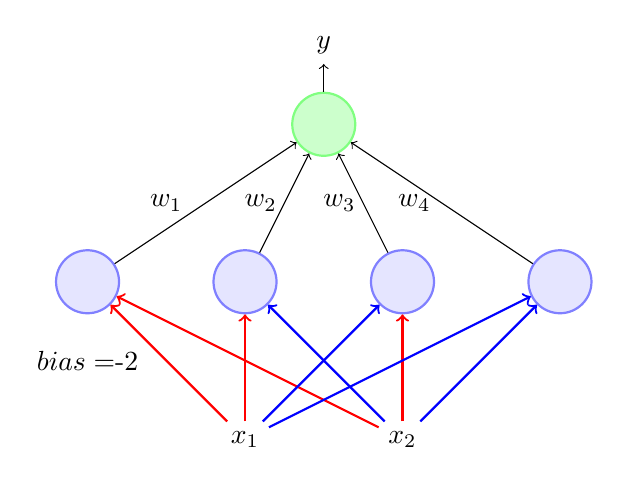
\begin{tikzpicture}
				\onslide<10->{\node [output_neuron] (out0) at (-3,12)  {} ;}

				\onslide<2->{\node (input0) at (-4,8)  {$x_1$};}
				\onslide<2->{\node (input1) at (-2,8) {$x_2$};}

				\onslide<2->{\node [hidden_neuron] (hi0) at (-6,10)  {  } ;}
				\onslide<2->{\node [hidden_neuron] (hi1) at (-4,10)  {  } ;}
				\onslide<2->{\node [hidden_neuron] (hi2) at (-2,10)  {  } ;}
				\onslide<2->{\node [hidden_neuron] (hi3) at (0,10)  {  } ;}



				\onslide<9->{\node (bias) at (-6,9)  {$bias=$-2} ;}

				\onslide<13->{\node (output0) at (-3,13)  {$y$} ;}

				\onslide<12->{\node (w1) at (-5,11)  {$w_1$} ;}
				\onslide<12->{\node (w2) at (-3.8,11)  {$w_2$} ;}
				\onslide<12->{\node (w3) at (-2.8,11)  {$w_3$} ;}
				\onslide<12->{\node (w4) at (-1.85,11)  {$w_4$} ;}

				\onslide<5->{\draw [->, thick, red] (input0) -- (hi0);}
				\onslide<5->{\draw [->, thick, red] (input1) -- (hi0);}

				\onslide<6->{\draw [->, thick, red](input0) -- (hi1);}
				\onslide<6->{\draw [->, thick, blue](input1) -- (hi1);}

				\onslide<7->{\draw [->, thick, blue] (input0) -- (hi2);}
				\onslide<7->{\draw [->, thick, red] (input1) -- (hi2);}

				\onslide<8->{\draw [->, thick, blue](input0) -- (hi3);}
				\onslide<8->{\draw [->, thick, blue](input1) -- (hi3);}

				\onslide<11->{\draw [->] (hi0) -- (out0);}
				\onslide<11->{\draw [->] (hi1) -- (out0);}
				\onslide<11->{\draw [->] (hi2) -- (out0);}
				\onslide<11->{\draw [->] (hi3) -- (out0);}

				\onslide<13->{\draw [->] (out0) -- (output0);}

				%\node at (-6,1) {red edge indicates $w$ = -1};
				%\node at (-6,0) {green edge indicates $w$ = +1};

			\end{tikzpicture}
			\onslide<4->{red edge indicates $w$ = -1 \\}
			\onslide<4->{blue edge indicates $w$ = +1}


		\end{overlayarea}

		\column{0.55\textwidth}
		\begin{overlayarea}{\textwidth}{\textheight}
			\only<1-13>{
				\begin{itemize}\justifying
					\item For this discussion, we will assume True = +1 and False = -1
					\item<2-> We consider 2 inputs and 4 perceptrons
					\item<3-> Each input is connected to all the 4 perceptrons with specific weights
					\item<9-> The bias ($w_0$) of each perceptron is -2 (i.e., each perceptron will fire only if the weighted sum of its input is $\geq$ 2)
					\item<10-> Each of these perceptrons is connected to an output perceptron by weights (which need to be learned)
					\item<13> The output of this perceptron ($y$) is the output of this network
				\end{itemize}
			}



		\end{overlayarea}
	\end{columns}

\end{frame}


\begin{frame}
	\begin{columns}

		\column{0.45\textwidth}
		\begin{overlayarea}{\textwidth}{\textheight}

			\vspace{1cm}

			\tikzstyle{input_neuron}=[circle,draw=red!50,fill=orange!10,thick,minimum size=10mm]
			\tikzstyle{hidden_neuron}=[circle,draw=blue!50,fill=blue!10,thick,minimum size=10mm]
			\tikzstyle{output_neuron}=[circle,draw=green!50,fill=green!20,thick,minimum size=10mm]

			\tikzstyle{input}=[circle,draw=black!50,fill=black!20,thick,minimum size=10mm]

			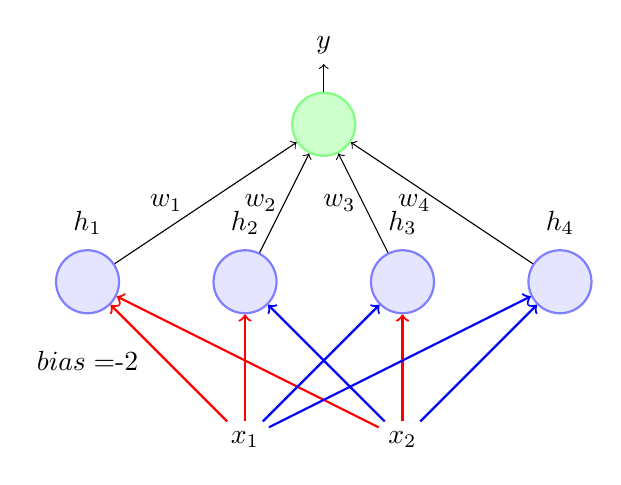
\begin{tikzpicture}
				\node [output_neuron] (out0) at (-3,12)  {} ;

				\node (input0) at (-4,8)  {$x_1$};
				\node (input1) at (-2,8) {$x_2$};

				\node [hidden_neuron] (hi0) at (-6,10)  {  } ;
				\node [hidden_neuron] (hi1) at (-4,10)  {  } ;
				\node [hidden_neuron] (hi2) at (-2,10)  {  } ;
				\node [hidden_neuron] (hi3) at (0,10)  {  } ;


				\onslide<5->{\node (h1_label) at (-6,10.75)  { $h_1$ } ;}
				\onslide<5->{\node (h2_label) at (-4,10.75)  { $h_2$ } ;}
				\onslide<5->{\node (h3_label) at (-2,10.75)  { $h_3$ } ;}
				\onslide<5->{\node (h4_label) at (-0,10.75)  { $h_4$ } ;}

				\node (bias) at (-6,9)  {$bias=$-2} ;

				\node (output0) at (-3,13)  {$y$} ;

				\node (w1) at (-5,11)  {$w_1$} ;
				\node (w2) at (-3.8,11)  {$w_2$} ;
				\node (w3) at (-2.8,11)  {$w_3$} ;
				\node (w4) at (-1.85,11)  {$w_4$} ;

				\draw [->, thick, red] (input0) -- (hi0);
				\draw [->, thick, red] (input1) -- (hi0);

				\draw [->, thick, red](input0) -- (hi1);
				\draw [->, thick, blue](input1) -- (hi1);

				\draw [->, thick, blue] (input0) -- (hi2);
				\draw [->, thick, red] (input1) -- (hi2);

				\draw [->, thick, blue](input0) -- (hi3);
				\draw [->, thick, blue](input1) -- (hi3);

				\draw [->] (hi0) -- (out0);
				\draw [->] (hi1) -- (out0);
				\draw [->] (hi2) -- (out0);
				\draw [->] (hi3) -- (out0);

				\draw [->] (out0) -- (output0);

				%\node at (-6,1) {red edge indicates $w$ = -1};
				%\node at (-6,0) {green edge indicates $w$ = +1};

			\end{tikzpicture}
			red edge indicates $w$ = -1 \\
			blue edge indicates $w$ = +1


		\end{overlayarea}

		\column{0.55\textwidth}
		\begin{overlayarea}{\textwidth}{\textheight}

			\textbf{Terminology:}
			\begin{itemize}\justifying
				\item This network contains 3 layers
				\item<2-> The layer containing the inputs ($x_1, x_2$) is called the \textbf{input layer}
				\item<3-> The middle layer containing the 4 perceptrons is called the \textbf{hidden layer}
				\item<4-> The final layer containing one output neuron is called the \textbf{output layer}
				\item<5-> The outputs of the 4 perceptrons in the hidden layer are denoted by $h_1, h_2, h_3, h_4$
				\item<6-> The red and blue edges are called layer 1 weights
				\item<7-> $w_1, w_2, w_3, w_4$ are called layer 2 weights


			\end{itemize}
		\end{overlayarea}
	\end{columns}

\end{frame}


\begin{frame}
	\begin{columns}

		\column{0.45\textwidth}
		\begin{overlayarea}{\textwidth}{\textheight}

			\vspace{1cm}

			\tikzstyle{input_neuron}=[circle,draw=red!50,fill=orange!10,thick,minimum size=10mm]
			\tikzstyle{hidden_neuron}=[circle,draw=blue!50,fill=blue!10,thick,minimum size=10mm]
			\tikzstyle{output_neuron}=[circle,draw=green!50,fill=green!20,thick,minimum size=10mm]

			\tikzstyle{input}=[circle,draw=black!50,fill=black!20,thick,minimum size=10mm]

			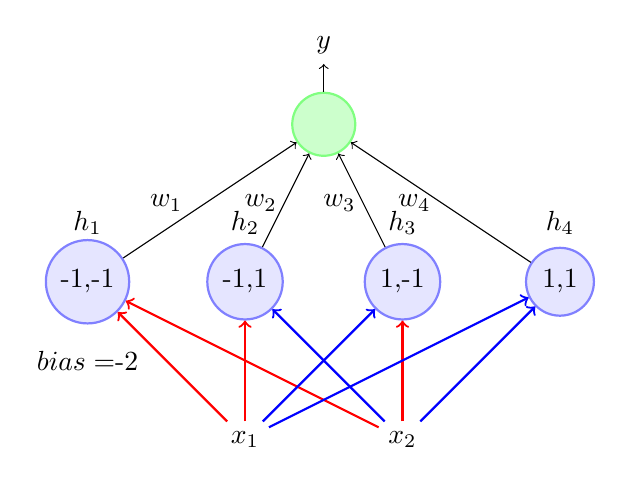
\begin{tikzpicture}
				\node [output_neuron] (out0) at (-3,12)  {} ;

				\node (input0) at (-4,8)  {$x_1$};
				\node (input1) at (-2,8) {$x_2$};

				\node [hidden_neuron] (hi0) at (-6,10)  {  } ;
				\node [hidden_neuron] (hi1) at (-4,10)  {  } ;
				\node [hidden_neuron] (hi2) at (-2,10)  {  } ;
				\node [hidden_neuron] (hi3) at (0,10)  {  } ;

				\node (h1_label) at (-6,10.75)  { $h_1$ } ;
				\node (h2_label) at (-4,10.75)  { $h_2$ } ;
				\node (h3_label) at (-2,10.75)  { $h_3$ } ;
				\node (h4_label) at (-0,10.75)  { $h_4$ } ;

				\onslide<6->{\node [hidden_neuron] (hi0) at (-6,10)  { -1,-1 } ;}
				\onslide<7->{\node [hidden_neuron] (hi1) at (-4,10)  { -1,1 } ;}
				\onslide<8->{\node [hidden_neuron] (hi2) at (-2,10)  { 1,-1 } ;}
				\onslide<9->{\node [hidden_neuron] (hi3) at (0,10)  { 1,1 } ;}


				\node (bias) at (-6,9)  {$bias=$-2} ;

				\node (output0) at (-3,13)  {$y$} ;

				\node (w1) at (-5,11)  {$w_1$} ;
				\node (w2) at (-3.8,11)  {$w_2$} ;
				\node (w3) at (-2.8,11)  {$w_3$} ;
				\node (w4) at (-1.85,11)  {$w_4$} ;

				\draw [->, thick, red] (input0) -- (hi0);
				\draw [->, thick, red] (input1) -- (hi0);

				\draw [->, thick, red](input0) -- (hi1);
				\draw [->, thick, blue](input1) -- (hi1);

				\draw [->, thick, blue] (input0) -- (hi2);
				\draw [->, thick, red] (input1) -- (hi2);

				\draw [->, thick, blue](input0) -- (hi3);
				\draw [->, thick, blue](input1) -- (hi3);

				\draw [->] (hi0) -- (out0);
				\draw [->] (hi1) -- (out0);
				\draw [->] (hi2) -- (out0);
				\draw [->] (hi3) -- (out0);

				\draw [->] (out0) -- (output0);

				%\node at (-6,1) {red edge indicates $w$ = -1};
				%\node at (-6,0) {green edge indicates $w$ = +1};

			\end{tikzpicture}
			red edge indicates $w$ = -1 \\
			blue edge indicates $w$ = +1


		\end{overlayarea}

		\column{0.55\textwidth}
		\begin{overlayarea}{\textwidth}{\textheight}

			\only<1->{
				\begin{itemize}\justifying
					\item We claim that this network can be used to implement \textbf{any} boolean function (linearly separable or not) !
					\item<2-> In other words, we can find $w_1, w_2, w_3, w_4$ such that the truth table of any boolean function can be represented by this network
					\item<3-> Astonishing claim! \onslide<4->{Well, not really, if you understand what is going on}
					\item<5-> Each perceptron in the middle layer fires only for a specific input (and no two perceptrons fire for the same input)
					      \only<6>{\item the first perceptron fires for \{-1,-1\} }
					      \only<7>{\item the second perceptron fires for \{-1,1\} }
					      \only<8>{\item the third perceptron fires for \{1,-1\} }
					      \only<9>{\item the fourth perceptron fires for \{1,1\} }
					\item<10-> Let us see why this network works by taking an example of the XOR function
				\end{itemize}
			}


		\end{overlayarea}
	\end{columns}

\end{frame}


\begin{frame}
	\begin{columns}

		\column{0.45\textwidth}
		\begin{overlayarea}{\textwidth}{\textheight}

			\vspace{1cm}

			\tikzstyle{input_neuron}=[circle,draw=red!50,fill=orange!10,thick,minimum size=10mm]
			\tikzstyle{hidden_neuron}=[circle,draw=blue!50,fill=blue!10,thick,minimum size=10mm]
			\tikzstyle{output_neuron}=[circle,draw=green!50,fill=green!20,thick,minimum size=10mm]

			\tikzstyle{input}=[circle,draw=black!50,fill=black!20,thick,minimum size=10mm]

			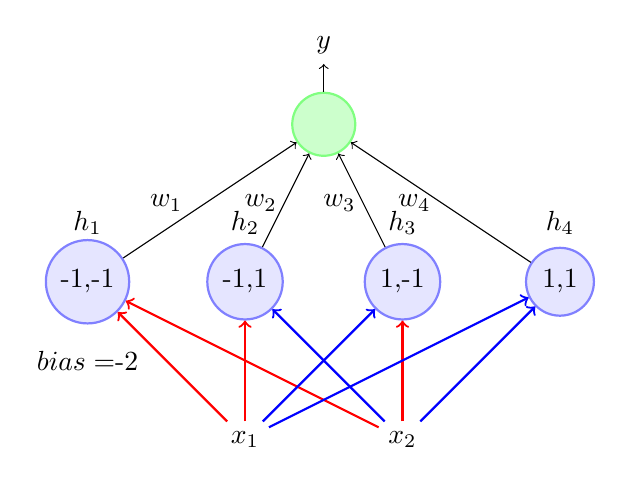
\begin{tikzpicture}
				\node [output_neuron] (out0) at (-3,12)  {} ;

				\node (input0) at (-4,8)  {$x_1$};
				\node (input1) at (-2,8) {$x_2$};

				\node [hidden_neuron] (hi0) at (-6,10)  {  } ;
				\node [hidden_neuron] (hi1) at (-4,10)  {  } ;
				\node [hidden_neuron] (hi2) at (-2,10)  {  } ;
				\node [hidden_neuron] (hi3) at (0,10)  {  } ;

				\node (h1_label) at (-6,10.75)  { $h_1$ } ;
				\node (h2_label) at (-4,10.75)  { $h_2$ } ;
				\node (h3_label) at (-2,10.75)  { $h_3$ } ;
				\node (h4_label) at (-0,10.75)  { $h_4$ } ;

				\node [hidden_neuron] (hi0) at (-6,10)  { -1,-1 } ;
				\node [hidden_neuron] (hi1) at (-4,10)  { -1,1 } ;
				\node [hidden_neuron] (hi2) at (-2,10)  { 1,-1 } ;
				\node [hidden_neuron] (hi3) at (0,10)  { 1,1 } ;


				\node (bias) at (-6,9)  {$bias=$-2} ;

				\node (output0) at (-3,13)  {$y$} ;

				\node (w1) at (-5,11)  {$w_1$} ;
				\node (w2) at (-3.8,11)  {$w_2$} ;
				\node (w3) at (-2.8,11)  {$w_3$} ;
				\node (w4) at (-1.85,11)  {$w_4$} ;

				\draw [->, thick, red] (input0) -- (hi0);
				\draw [->, thick, red] (input1) -- (hi0);

				\draw [->, thick, red](input0) -- (hi1);
				\draw [->, thick, blue](input1) -- (hi1);

				\draw [->, thick, blue] (input0) -- (hi2);
				\draw [->, thick, red] (input1) -- (hi2);

				\draw [->, thick, blue](input0) -- (hi3);
				\draw [->, thick, blue](input1) -- (hi3);

				\draw [->] (hi0) -- (out0);
				\draw [->] (hi1) -- (out0);
				\draw [->] (hi2) -- (out0);
				\draw [->] (hi3) -- (out0);

				\draw [->] (out0) -- (output0);

				%\node at (-6,1) {red edge indicates $w$ = -1};
				%\node at (-6,0) {green edge indicates $w$ = +1};

			\end{tikzpicture}
			red edge indicates $w$ = -1 \\
			blue edge indicates $w$ = +1


		\end{overlayarea}

		\column{0.55\textwidth}
		\begin{overlayarea}{\textwidth}{\textheight}

			\begin{itemize}\justifying
				\item Let $w_0$ be the bias output of the neuron (\textit{i.e.}, it will fire if $\sum_{i=1}^{4}w_ih_i \geq w_0$)
			\end{itemize}

			\onslide<2->{
				\small{
					\begin{table}
						\begin{tabular}{cccccccc}
							\hline
							\onslide<2->{$x_1$} & \onslide<2->{$x_2$} & \onslide<2->{$XOR$} & \onslide<2->{$h_1$} & \onslide<2->{$h_2$} & \onslide<2->{$h_3$} & \onslide<2->{$h_4$} & \onslide<2->{$\sum_{i=1}^{4}w_ih_i$} \\
							\hline
							\onslide<2->{0}     & \onslide<2->{0}     & \onslide<2->{0}     & \onslide<2->{1}     & \onslide<2->{0}     & \onslide<2->{0}     & \onslide<2->{0}     & \onslide<2->{$w_1$}                  \\
							\onslide<3->{0}     & \onslide<3->{1}     & \onslide<3->{1}     & \onslide<3->{0}     & \onslide<3->{1}     & \onslide<3->{0}     & \onslide<3->{0}     & \onslide<3->{$w_2$}                  \\
							\onslide<4->{1}     & \onslide<4->{0}     & \onslide<4->{1}     & \onslide<4->{0}     & \onslide<4->{0}     & \onslide<4->{1}     & \onslide<4->{0}     & \onslide<4->{$w_3$}                  \\
							\onslide<5->{1}     & \onslide<5->{1}     & \onslide<5->{0}     & \onslide<5->{0}     & \onslide<5->{0}     & \onslide<5->{0}     & \onslide<5->{1}     & \onslide<5->{$w_4$}                  \\
							\hline
						\end{tabular}
					\end{table}
				}
			}
			\vspace{-0.2in}
			\textnormal{
				\begin{itemize}\justifying
					\item<6-> This results in the following four conditions to implement XOR: $w_1 < w_0, w_2 \geq w_0, w_3 \geq w_0, w_4 < w_0$
					\item<7-> Unlike before, there are no contradictions now and the system of inequalities can be satisfied
					\item<8-> Essentially each $w_i$ is now responsible for one of the 4 possible inputs and can be adjusted to get the desired output for that input
				\end{itemize}
			}
		\end{overlayarea}
	\end{columns}

\end{frame}




\begin{frame}
	\begin{columns}

		\column{0.45\textwidth}
		\begin{overlayarea}{\textwidth}{\textheight}

			\vspace{1cm}

			\tikzstyle{input_neuron}=[circle,draw=red!50,fill=orange!10,thick,minimum size=10mm]
			\tikzstyle{hidden_neuron}=[circle,draw=blue!50,fill=blue!10,thick,minimum size=10mm]
			\tikzstyle{output_neuron}=[circle,draw=green!50,fill=green!20,thick,minimum size=10mm]

			\tikzstyle{input}=[circle,draw=black!50,fill=black!20,thick,minimum size=10mm]

			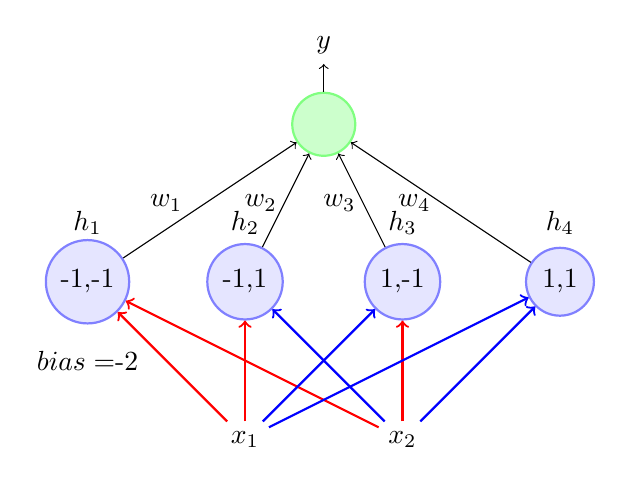
\begin{tikzpicture}
				\node [output_neuron] (out0) at (-3,12)  {} ;

				\node (input0) at (-4,8)  {$x_1$};
				\node (input1) at (-2,8) {$x_2$};

				\node [hidden_neuron] (hi0) at (-6,10)  {  } ;
				\node [hidden_neuron] (hi1) at (-4,10)  {  } ;
				\node [hidden_neuron] (hi2) at (-2,10)  {  } ;
				\node [hidden_neuron] (hi3) at (0,10)  {  } ;

				\node (h1_label) at (-6,10.75)  { $h_1$ } ;
				\node (h2_label) at (-4,10.75)  { $h_2$ } ;
				\node (h3_label) at (-2,10.75)  { $h_3$ } ;
				\node (h4_label) at (-0,10.75)  { $h_4$ } ;

				\node [hidden_neuron] (hi0) at (-6,10)  { -1,-1 } ;
				\node [hidden_neuron] (hi1) at (-4,10)  { -1,1 } ;
				\node [hidden_neuron] (hi2) at (-2,10)  { 1,-1 } ;
				\node [hidden_neuron] (hi3) at (0,10)  { 1,1 } ;


				\node (bias) at (-6,9)  {$bias=$-2} ;

				\node (output0) at (-3,13)  {$y$} ;

				\node (w1) at (-5,11)  {$w_1$} ;
				\node (w2) at (-3.8,11)  {$w_2$} ;
				\node (w3) at (-2.8,11)  {$w_3$} ;
				\node (w4) at (-1.85,11)  {$w_4$} ;

				\draw [->, thick, red] (input0) -- (hi0);
				\draw [->, thick, red] (input1) -- (hi0);

				\draw [->, thick, red](input0) -- (hi1);
				\draw [->, thick, blue](input1) -- (hi1);

				\draw [->, thick, blue] (input0) -- (hi2);
				\draw [->, thick, red] (input1) -- (hi2);

				\draw [->, thick, blue](input0) -- (hi3);
				\draw [->, thick, blue](input1) -- (hi3);

				\draw [->] (hi0) -- (out0);
				\draw [->] (hi1) -- (out0);
				\draw [->] (hi2) -- (out0);
				\draw [->] (hi3) -- (out0);

				\draw [->] (out0) -- (output0);

				%\node at (-6,1) {red edge indicates $w$ = -1};
				%\node at (-6,0) {green edge indicates $w$ = +1};

			\end{tikzpicture}
			red edge indicates $w$ = -1 \\
			blue edge indicates $w$ = +1


		\end{overlayarea}

		\column{0.55\textwidth}
		\begin{overlayarea}{\textwidth}{\textheight}

			\begin{itemize}\justifying
				\item<1-> It should be clear that the same network can be used to represent the remaining 15 boolean functions also
				\item<2-> Each boolean function will result in a different set of non-contradicting inequalities which can be satisfied by appropriately setting $w_1, w_2, w_3, w_4$
				\item<3-> Try it!
			\end{itemize}

		\end{overlayarea}
	\end{columns}

\end{frame}

\begin{frame}
	\begin{itemize}\justifying
		\item<1-> What if we have more than 3 inputs ?
	\end{itemize}
\end{frame}


\begin{frame}
	\begin{itemize}\justifying
		\item Again each of the 8 perceptorns will fire only for one of the 8 inputs
		\item Each of the 8 weights in the second layer is responsible for one of the 8 inputs and can be adjusted to produce the desired output for that input
	\end{itemize}

	\tikzstyle{input_neuron}=[circle,draw=red!50,fill=orange!10,thick,minimum size=8mm]
	\tikzstyle{hidden_neuron}=[circle,draw=blue!50,fill=blue!10,thick,minimum size=8mm]
	\tikzstyle{output_neuron}=[circle,draw=green!50,fill=green!20,thick,minimum size=8mm]

	\tikzstyle{input}=[circle,draw=black!50,fill=black!20,thick,minimum size=10mm]

	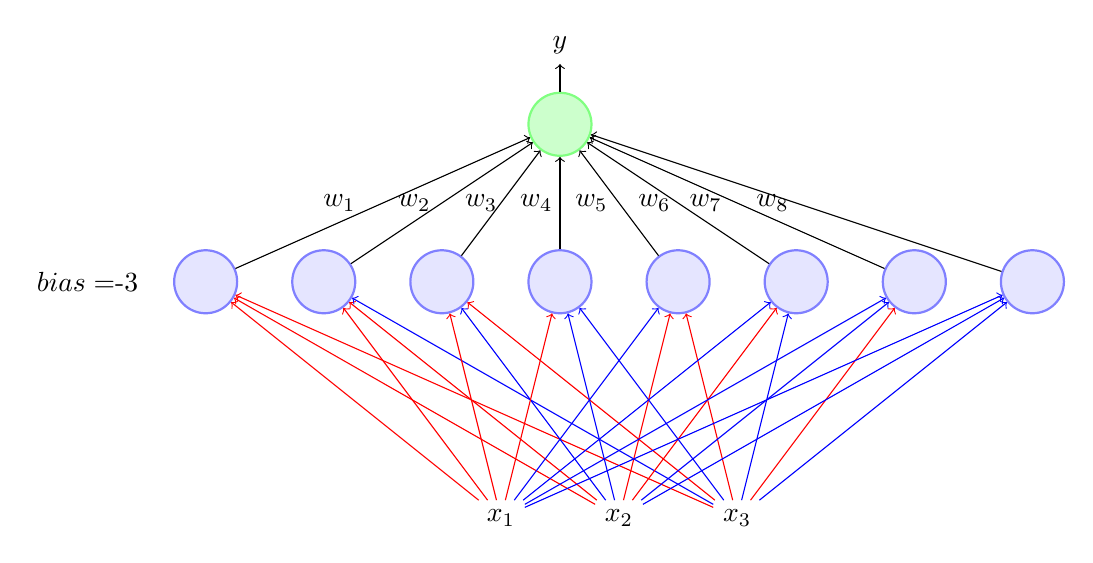
\begin{tikzpicture}
		\node [output_neuron] (out0) at (0,12)  {} ;

		\node (input0) at (-0.75,7)  {$x_1$};
		\node (input1) at (0.75,7) {$x_2$};
		\node (input2) at (2.25,7) {$x_3$};

		\node [hidden_neuron] (hi0) at (-4.5,10)  {  } ;
		\node [hidden_neuron] (hi1) at (-3,10)  {  } ;
		\node [hidden_neuron] (hi2) at (-1.5,10)  {  } ;
		\node [hidden_neuron] (hi3) at (0,10)  {  } ;
		\node [hidden_neuron] (hi4) at (1.5,10)  {  } ;
		\node [hidden_neuron] (hi5) at (3,10)  {  } ;
		\node [hidden_neuron] (hi6) at (4.5,10)  {  } ;
		\node [hidden_neuron] (hi7) at (6,10)  {  } ;



		\node (bias) at (-6,10)  {$bias=$-3} ;

		\node (output0) at (0,13)  {$y$} ;

		\node (w1) at (-2.8,11)  {$w_1$} ;
		\node (w2) at (-1.85,11)  {$w_2$} ;
		\node (w3) at (-1.0,11)  {$w_3$} ;
		\node (w3) at (-0.3,11)  {$w_4$} ;
		\node (w3) at (0.4,11)  {$w_5$} ;
		\node (w3) at (1.2,11)  {$w_6$} ;
		\node (w4) at (1.85,11)  {$w_7$} ;
		\node (w4) at (2.7,11)  {$w_8$} ;

		\draw [->,  red] (input0) -- (hi0);
		\draw [->,  red] (input1) -- (hi0);
		\draw [->,  red] (input2) -- (hi0);

		\draw [->,  red](input0) -- (hi1);
		\draw [->,  red](input1) -- (hi1);
		\draw [->,  blue] (input2) -- (hi1);

		\draw [->,  red] (input0) -- (hi2);
		\draw [->,  blue] (input1) -- (hi2);
		\draw [->,  red] (input2) -- (hi2);

		\draw [->,  red](input0) -- (hi3);
		\draw [->,  blue](input1) -- (hi3);
		\draw [->,  blue] (input2) -- (hi3);

		\draw [->,  blue](input0) -- (hi4);
		\draw [->,  red](input1) -- (hi4);
		\draw [->,  red] (input2) -- (hi4);

		\draw [->,  blue](input0) -- (hi5);
		\draw [->,  red](input1) -- (hi5);
		\draw [->,  blue] (input2) -- (hi5);

		\draw [->,  blue](input0) -- (hi6);
		\draw [->,  blue](input1) -- (hi6);
		\draw [->,  red] (input2) -- (hi6);

		\draw [->,  blue](input0) -- (hi7);
		\draw [->,  blue](input1) -- (hi7);
		\draw [->,  blue] (input2) -- (hi7);

		\draw [->] (hi0) -- (out0);
		\draw [->] (hi1) -- (out0);
		\draw [->] (hi2) -- (out0);
		\draw [->] (hi3) -- (out0);
		\draw [->] (hi4) -- (out0);
		\draw [->] (hi5) -- (out0);
		\draw [->] (hi6) -- (out0);
		\draw [->] (hi7) -- (out0);

		\draw [->] (out0) -- (output0);

		%\node at (-6,1) {red edge indicates $w$ = -1};
		%\node at (-6,0) {green edge indicates $w$ = +1};

	\end{tikzpicture}
	%\begin{itemize}\justifying
	%\item red edge indicates $w$ = -1
	%\item blue edge indicates $w$ = +1
	%\end{itemize}
\end{frame}


\begin{frame}
	\begin{itemize}\justifying
		\item<1-> What if we have $n$ inputs ?
	\end{itemize}
\end{frame}

\begin{frame}
	\begin{block}{Theorem}
		\justifying
		Any boolean function of $n$ inputs can be represented exactly by a network of perceptrons containing 1 hidden layer with $2^n$ perceptrons and one output layer containing $1$ perceptron \\
		\vspace{0.2in}
		\onslide<2->{\textbf{Proof (informal:)} We just saw how to construct such a network} \\
		\vspace{0.2in}
		\onslide<2->{\textbf{Note:} A network of $2^n + 1$ perceptrons is not necessary but sufficient. For example, we already saw how to represent AND function with just 1 perceptron}\\
		\vspace{0.2in}
		\onslide<3->{\textbf{Catch:} As $n$ increases the number of perceptrons in the hidden layers obviously increases exponentially}
	\end{block}
\end{frame}


\begin{frame}
	\begin{block}{The story so far ...}
		\begin{itemize}\justifying
			\item<1-> Networks of the form that we just saw (containing, an input, output and one or more hidden layers) are called Multilayer Perceptrons (MLP, in short)
			\item<2-> More appropriate terminology would be``Multilayered Network of Perceptrons'' but MLP is the more commonly used name
			\item<3-> The theorem that we just saw gives us the representation power of a MLP with a single hidden layer
			\item<4-> Specifically, it tells us that a MLP with a single hidden layer can represent \textbf{any} boolean function
		\end{itemize}
	\end{block}
\end{frame}


\end{document}


